\begin{figure}[h!]\label{fig:location}
	\centering
	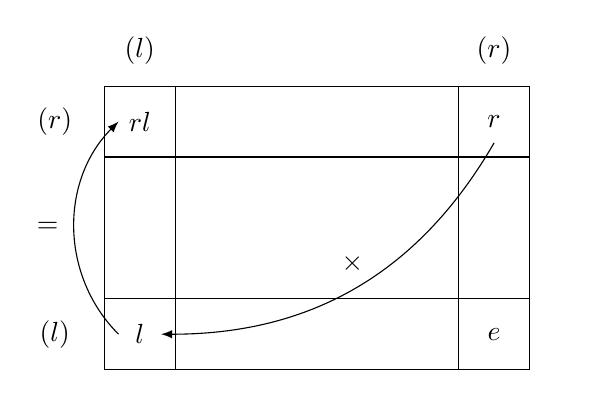
\begin{tikzpicture}[scale = 0.9]
	\tikzstyle{fleche}=[->,>=latex,rounded corners=4pt]
	\node at (0,0){$l$};
	\node at (0,3){$rl$};
	\node at (5,0){$e$};
	\node at (5,3){$r$};
	\draw (-.5,3.5) -- (-.5, -.5);
	\draw (.5,3.5) -- (.5, -.5);
	\draw (5.5,3.5) -- (5.5, -.5);
	\draw (4.5,3.5) -- (4.5, -.5);
	\draw (-.5,3.5) -- (5.5, 3.5);
	\draw (-.5,2.5) -- (5.5, 2.5);
	\draw (-.5,.5) -- (5.5, .5);
	\draw (-.5,-.5) -- (5.5, -.5);
	
	\draw[->, >=latex, bend left = 45] (-.3, 0) to (-.3, 3);
	\node at (-1.3, 1.5){$=$};
	\draw[->, >=latex, bend left] (5,2.7) to (0.3,0);
	\node at (3, 1){$\times$};
	
	\node at (-1.2, 3){$\rc(r)$};
	\node at (-1.2, 0){$\rc(l)$};
	\node at (0, 4){$\lc(l)$};
	\node at (5, 4){$\lc(r)$};
	\node at (6, 0){};
	
	\end{tikzpicture}
	\caption{Location Theorem\\ {\small Since there is an idempotent $e$ in $\lc(r)\cap \rc(l)$, $rl$ stays in the same $\jc$-class, in $\lc(l) \cap \rc(r)$.}}
\end{figure}